\chapter{Flujo Compresible}

	
	En las sesiones introductorias del curso vimos que el criterio de
	compresibilidad relacionaba la presión con la velocidad del flujo.
	Para el aire la velocidad a partir de la cual el flujo puede y debe
	ser considerado compresible está alrededor de $40~\text{m/s}$. Teóricamente
	también los líquidos en ciertas condiciones pueden ser considerados
	compresibles. Pero estas condiciones son dificiles de conseguir en
	la práctica (unos $200~\text{m/s}$ y/o más de $200~\text{atm}$).
	
	En el estudio de flujo compresible tiene un papel importante la termodinámica
	del proceso.
	
	El parámetro más importante en el estudio del flujo compresible es
	el número de Mach, 
	
\begin{equation}
		\ma=\frac{u}{c}
\end{equation}
	
	donde $c$ es la velocidad del sonido es el fluido, que depende,
	como veremos de la temperatura del fluido.


\section{Repaso de Termodinámica}

	
	La variación de entropí a se calcula a partir de las dos primeras
	leyes de la Termodinámica, que, para un gas perfecto, da 
	
\begin{equation}
		T\dif s=\dif h-\frac{\dif p}{\rho}=c_{p}\dif T-\frac{\dif p}{\rho}
\end{equation}
	
	
	Dado que 
	\[
	\frac{p}{\rho}=rT\,;\,\text{con }r=\frac{R}{M}=c_{p}-c_{v},
	\]
	
	\[
	\dif s=c_{p}\frac{\dif T}{T}-r\frac{\dif p}{p}
	\]
	
	\[
	\Rightarrow\,\int_{1}^{2}\dif s=\int_{1}^{2}c_{p}\frac{\dif T}{T}-r\ln\frac{p_{2}}{p_{1}}
	\]
	
	
	Si $c_{p}$ es variable, la integral se resuelve de forma numérica
	o con la ayuda de tablas. Si puede ser considerada constante, 
	
\begin{equation}
		s_{2}-s_{1}=c_{p}\ln\frac{T_{2}}{T_{1}}-r\ln\frac{p_{2}}{p_{1}}
\end{equation}
	
	
	Si realizamos el mismo cálculo, pero a partir de $\dif s=c_{v}\dif T-p\dif\frac{1}{\rho}$
	habríamos llegado a 
	
\begin{equation}
		s_{2}-s_{1}=c_{v}\ln\frac{T_{2}}{T_{1}}-r\ln\frac{\rho_{2}}{\rho_{1}}
\end{equation}
	
	
	Estas relaciones nos permiten calcular la variación de entropía en
	procesos no isoentrópicos, como puede ser, por ejemplo el frente de
	una onda de choque.
	
	Si el proceso es isoentrópico, $s_{2}-s_{1}=0$ y podemos escribir
	las conocidas relaciones 
	
\begin{equation}
		\frac{p_{2}}{p_{1}}=\left(\frac{\rho_{2}}{\rho_{1}}\right)^{\gamma}=\left(\frac{T_{2}}{T_{1}}\right)^{\frac{\gamma}{\gamma-1}}\;\text{con }\;\gamma=\frac{c_{p}}{c_{v}}
\end{equation}
	
	

\section{La velocidad del sonido}

	
	El sonido no es más que una onda de presión de amplitud pequeña.
	
	\medskip{}
	
	\begin{tabular}{cc}
		\begin{minipage}[c]{0.3\textwidth}%
			\begin{center}
				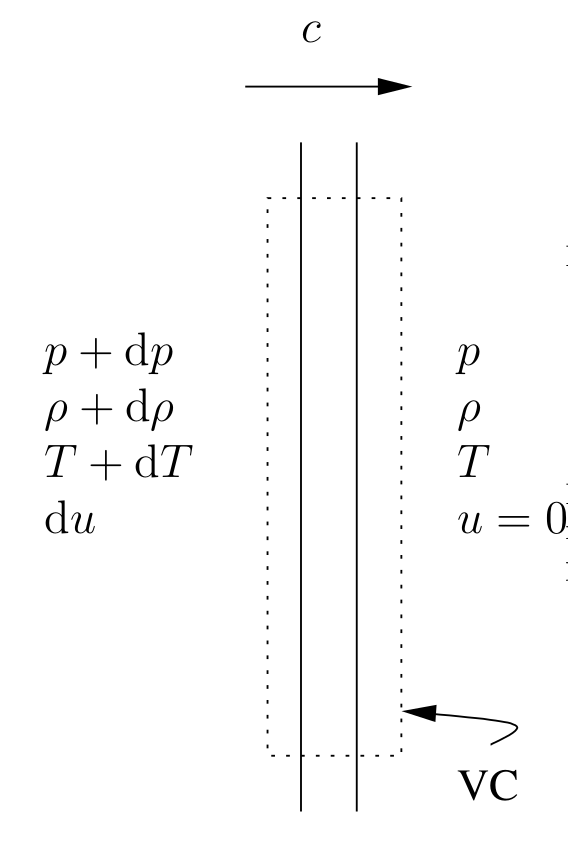
\includegraphics[width=\linewidth]{TeX_files/chapter11-Compresible/onda1}
			\end{center}
		
		\end{minipage} & %
		\begin{minipage}[c]{0.6\textwidth}%
			Por continuidad, 
			\[
			\int_{SC}\rho\vec{u}_{r}\cdot\dif\vec{S}=-\rho cA+(\rho+\Delta\rho)(c-\Delta u)A=0
			\]
			
			\[
			\Rightarrow\,\Delta u=c\,\frac{\Delta\rho}{\rho+\Delta\rho}
			\]
			
			Dado que no hay gradiente de velocidad en la dirección normal al flujo,
			no hay fricción, y la conservación de la cantidad de movimiento nos
			permite relacionar la velocidad de la onda con la variación de presión %
		\end{minipage}\tabularnewline
	\end{tabular}

	
	\[
	-\Delta pA=\dot{m}(u_{2}-u_{1})=\rho Ac(-\Delta u)\,\Rightarrow\,\Delta p=\rho c\Delta u
	\]
	
	\[
	\Delta p=\rho c\left[c\,\frac{\Delta\rho}{\rho+\Delta\rho}\right]=c^{2}\,\frac{\rho\Delta\rho}{\rho+\Delta\rho}
	\]
	
	\[
	\Rightarrow c^{2}=\frac{\Delta p}{\Delta\rho}\left[1+\frac{\Delta\rho}{\rho}\right]
	\]
	
	En el límite $\Delta\rho\rightarrow0$, hablamos de velocidad del
	sonido, 
	
\begin{equation}
		\boxed{c=\sqrt{\dparc{p}{\rho}}}
\end{equation}
	
	
	
	Si el proceso es adiabático (no hay gradientes de temperatura en el interior
	o exterior de la onda) 
	\[
	c=\sqrt{\left.\dparc{p}{\rho}\right|_{s}}=\sqrt{\gamma\left.\dparc{p}{\rho}\right|_{T}}
	\]
	
	Para un gas perfecto, $\left.\dparc{p}{\rho}\right|_{T}=rT$, de forma
	que 
	\[
	c=\sqrt{\gamma rT}
	\]
	
	Para el aire, $\gamma=1.4$ y $r=287$, de forma que 
	\[
	c\approx20\sqrt{T}
	\]
	con $T$ en Kelvins y $c$ en m/s. A $20^{\circ}\,C$, $c\approx340\,\text{m/s}\approx1220\,\text{km/h}$


\section{Flujo adiabático}

	
	Ecuación de Bernoulli (la poca densidad del fluido hace que el término
	de gravedad sea menospreciable) 
	
\begin{equation}
		h+\frac{u^{2}}{2}=\text{cte}=h_{0}
\end{equation}
	
	
	$h_{0}$ : \textcolor{red}{entalpía de estancamiento}. Entalpía que
	obtendríamos en el fluido si lo llevásemos al reposo de forma adiabática.
	
	Para gases reales, el cálculo de la entalpía para una cierta temperatura
	debe realizarse con tablas. Para gases perfectos, $h=c_{p}T$, 
	
\begin{equation}
		c_{p}T+\frac{u^{2}}{2}=c_{p}T_{0}
\end{equation}
	
	
	$T_{0}$ : Temperatura de estancamiento
	
	Si la entalpía (o la temperatura) son llevados a cero de forma adiabática,
	la velocidad del flujo alcanza su valor máximo, 
	\[
	u_{max}=\sqrt{2h_{0}}
	\]
	
	\[
	u_{max}=\sqrt{2c_{p}T_{0}}\qquad\text{para un gas perfecto}
	\]
	
	Podemos obtener la \textcolor{blue}{forma adimensional de la ecuación
		de Bernoulli}, 
	
\begin{equation}
		1+\frac{u^{2}}{2c_{p}T}=\frac{T_{0}}{T}
\end{equation}
	
	o bien, usando $c_{p}T=\gamma rT/(\gamma-1)=c^{2}/(\gamma-1)$, 
	
\begin{equation}
		\boxed{1+\frac{\gamma-1}{2}\ma^{2}=\frac{T_{0}}{T}}
\end{equation}
		
	Dado que la velocidad del sonido es proporcional a $\sqrt{T}$, 
	
\begin{equation}
		\frac{c_{0}}{c}=\sqrt{\frac{T_{0}}{T}}=\left[1+\frac{\gamma-1}{2}\ma^{2}\right]^{1/2}
\end{equation}
	
	
	Estas expresiones son válidas siempre que el flujo sea adiabático.
	Si, además, es isoentrópico (es decir, reversible), para un gas perfecto
	tenemos 
	\begin{eqnarray}
		\frac{p_{0}}{p}=\left(\frac{T_{0}}{T}\right)^{\frac{\gamma}{\gamma-1}}=\left[1+\frac{\gamma-1}{2}\ma^{2}\right]^{\frac{\gamma}{\gamma-1}}\\
		\frac{\rho_{0}}{\rho}=\left(\frac{T_{0}}{T}\right)^{\frac{1}{\gamma-1}}=\left[1+\frac{\gamma-1}{2}\ma^{2}\right]^{\frac{1}{\gamma-1}}
	\end{eqnarray}
	


\section{Valores sónicos}
	
	Además de $T_{0}$, $p_{0}$, $\rho_{0}$ y $c_{0}$, también son
	útiles los valores denominados \textcolor{red}{sónicos}, o \textcolor{red}{críticos}, obtenidos cuando $\ma=1.0$,
	
	 $p^{*}=p_{0}\left(\frac{2}{\gamma+1}\right)^{\frac{\gamma}{\gamma-1}};T^{*}=T_{0}\frac{2}{\gamma+1};\rho^{*}=\rho_{0}\left(\frac{2}{\gamma+1}\right)^{\frac{1}{\gamma-1}};c^{*}=c_{0}\left(\frac{2}{\gamma+1}\right)^{\frac{1}{2}}(=u^{*})$


	
	\textbf{Ejemplo :}
		\begin{tabular}{cc}
			\begin{minipage}[c]{0.5\textwidth}%
\begin{center}
	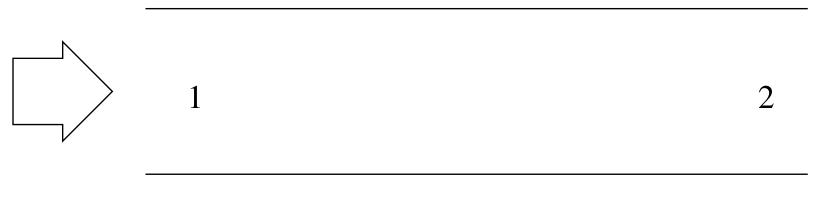
\includegraphics[width=1\linewidth]{TeX_files/chapter11-Compresible/ejemplo1}
\end{center}
Flujo adiabático de aire
			\end{minipage} & %
			\begin{minipage}[c]{0.4\textwidth}%
				
				\begin{eqnarray*}
					u_{1} & = & 240\,\text{m/s}\\
					T_{1} & = & 320\,\text{K}\\
					p_{1} & = & 170\,\text{kPa}
				\end{eqnarray*}
				%
			\end{minipage}\tabularnewline
		\end{tabular}

\bigskip
		
		Queremos calcular ${T_{0}}_{1}$, ${p_{0}}_{1}$, ${\rho_{0}}_{1}$,
		$\ma_{1}$, ${u_{max}}_{1}$ y $u_{1}^{*}$.
		
		Si $u_{2}=290\,\text{m/s}$ y $p_{2}=135\,\text{kPa}$, calcular ${p_{0}}_{2}$.
		
		Dado que no sabemos si el flujo es isoentrópico o no, sólo podemos
		usar las relaciones isoentrópicas para calcular $p_{0}$ y $\rho_{0}$
		de forma local en 1. {\footnotesize{}
			\begin{eqnarray*}
				r & = & 287\,\text{J/Kg\, K}\\
				\gamma & = & 1.4\\
				c_{p} & = & 1005\,\text{J/Kg\, K}
			\end{eqnarray*}
		}{\footnotesize\par}

		\begin{tabular}{c|c}
			\begin{minipage}[c]{0.45\textwidth}%
				Empezamos calculando Ma, {\footnotesize{}
					\[
					c_{1}=\sqrt{\gamma rT_{1}}=358.6\,\text{m/s}
					\]
					\[
					\Rightarrow\,\ma_{1}=\frac{240}{358.6}=0.67
					\]
					\[
					{T_{0}}_{1}=\left[1+\frac{\gamma-1}{2}\ma^{2}\right]T_{1}=348.7\,\text{K}
					\]
				}{\footnotesize\par}
				
				Otra forma de calcularlo habría sido con 
				\[
				{T_{0}}_{1}=T_{1}+\frac{u_{1}^{2}}{2c_{p}}
				\]
				%
			\end{minipage} & %
			\begin{minipage}[c]{0.45\textwidth}%
				{\footnotesize{}
					\begin{eqnarray*}
						{p_{0}}_{1} & = & p_{1}\left[1+\frac{\gamma-1}{2}\ma^{2}\right]^{\frac{\gamma}{\gamma-1}}=\\
						& = & 229.6\,\text{kPa}\\
						{\rho_{0}}_{1} & = & \frac{{p_{0}}_{1}}{r{T_{0}}_{1}}=2.29\,\text{Kg}/\text{m}^{3}\\
						{u_{max}}_{1} & = & \sqrt{2c_{p}{T_{0}}_{1}}=837.2\,\text{m/s}\\
						u_{1}^{*} & = & \sqrt{\frac{2}{\gamma+1}}{c_{0}}_{1}=\sqrt{\frac{2\gamma r{T_{0}}_{1}}{\gamma+1}}=\\
						& = & 342\,\text{m/s}
					\end{eqnarray*}
				} %
			\end{minipage}\tabularnewline
		\end{tabular}
		
		En el punto 2 podemos calcular la temperatura, dado que el flujo
		es adiabático y, por lo tanto, ${T_{0}}_{1}={T_{0}}_{2}$, 
		\[
		T_{2}={T_{0}}_{2}-\frac{u_{2}^{2}}{2c_{p}}=306.9\,\text{K}
		\]
		y la presión de estancamiento en 2 es 
		\[
		{p_{0}}_{2}=p_{2}\left(\frac{{T_{0}}_{2}}{T_{2}}\right)^{\frac{\gamma}{\gamma-1}}=211\,\text{kPa}
		\]

\subsection*{Actividad 1:}
		
		1.- ${p_{0}}_{2}<{p_{0}}_{1}$. ?`Porqué?
		
		2.- ¿Es el conducto de sección constante?
		
		3.- ¿Cuál es la variación de entropía?

